\documentclass[11pt]{article}

%%
%% PACKAGES
%%

\usepackage[margin=0.9in, top=0.8in, bottom=1.0in]{geometry}
\usepackage[charter]{mathdesign} % Main font
\usepackage[scaled]{beramono} % Lovely monospace font
\usepackage[T1]{fontenc}
%\usepackage{amsmath, amssymb}
\usepackage{mathtools}
\usepackage{mathdots}
\usepackage{titlesec} % Custom section headings.
\usepackage{microtype}
\usepackage{xcolor}
\usepackage{xspace}
\usepackage{xfrac}
\usepackage{calc}
\usepackage{subcaption}

% Graphics.
%\usepackage{graphicx}
\usepackage[update,prepend]{epstopdf} % To use eps files.

% Code listings.
\usepackage{listings} % Code listings.
\usepackage{matlab-prettifier} % MATLAB code listings

% Tweaks for captions and enumerations.
\usepackage[labelfont=bf]{caption} % Figure captions.
\usepackage{enumitem} % Fine tuning enumerations.
%\usepackage{floatrow} % Captions to the right of figures.

% Plotting and drawing
\usepackage{tikz} % This automatically loads graphicx!
\usetikzlibrary{calc} % For relative positions to defined coords
\usepackage{pgfplots} % Scientific plotting tools
\pgfplotsset{compat=1.7}

% Figure placement
\usepackage{wrapfig}
\captionsetup[wrapfigure]{margin=0.5cm}

% Packages to makes tables pretty.
\usepackage{array}
\usepackage{booktabs}
\setlength{\heavyrulewidth}{1.5pt}
\setlength{\abovetopsep}{4pt}

% Fancyhdr package stuff...
\usepackage{fancyhdr}
\setlength{\headheight}{0pt}
\setlength{\footskip}{50pt}
\renewcommand{\headrulewidth}{0pt}
\renewcommand{\footrulewidth}{0pt}

%%
%% SETTINGS
%%

% Path to look for graphics
\graphicspath{{../images/}}
%\epstopdfsetup{outdir=../images/}

% Caption spacing
\setlength{\abovecaptionskip}{0pt}

% List spacing
\setlist{noitemsep}

% Math operator font
\DeclareSymbolFont{sfoperators}{OT1}{cmss}{m}{n}
\DeclareSymbolFontAlphabet{\mathsf}{sfoperators}
\makeatletter
\def\operator@font{\mathgroup\symsfoperators}
\makeatother

%% No indent all paragraphs
%\setlength{\parindent}{0in}

% Figure references
\newcommand{\figref}[1]{Figure~\ref{#1}}

% Special format section headings
\titleformat{\section}%
	{\large\bf\scshape}% Text formatting
	{\arabic{section}}% Number
	{1em}% Space between number and text
	{}% Code before
	[]% Code after
\titleformat{\subsection}%
	{\normalsize\bf\scshape}% Text formatting
	{\arabic{section}.\arabic{subsection}}% Number
	{1em}% Space between number and text
	{}% Code before
	[]% Code after
%\titleformat{\subsubsection}%
%	{\color{blue}}% Text formatting
%	{\arabic{subsubsection} $\rightarrow$}% Number
%	{1em}% Space between number and text
%	{}% Code before
%	[]% Code after

\definecolor{mygray}{rgb}{0.4, 0.4, 0.4}
\lstset{
style=Matlab-editor,
mlscaleinline=false,
basicstyle=\ttfamily\lst@ifdisplaystyle\scriptsize\fi,
frame=single,
rulecolor=\color{mygray},
numbers=left,
numbersep=10pt,
numberstyle=\footnotesize \ttfamily \color{mygray},
xleftmargin=30pt,
xrightmargin=5pt,
framexleftmargin=4pt,
framextopmargin=2pt
}

% Allow white-space to be eaten within any lst environments between returns.
\lstset{breaklines,breakatwhitespace}

% Define the | chacacter as shorthand for inline listings.
\lstMakeShortInline{`}

%%
%% COMMANDS
%%

% Various plot lines to include in-line.
\newcommand{\solidrule}[1][8mm]{\rule[0.5ex]{#1}{1.5pt}}
\newcommand{\dashrule}{\mbox{%
	\solidrule[2mm]\hspace{1mm}\solidrule[2mm]\hspace{1mm}\solidrule[2mm]}}
\newcommand{\dotdashrule}{\mbox{%
	\solidrule[0.5mm]\hspace{1mm}\solidrule[2mm]\hspace{1mm}\solidrule[0.5mm]\hspace{1mm}\solidrule[2mm]}}

% Automated file inclusion for code listings
\makeatletter
\def\includecode{\@ifnextchar[{\@with}{\@without}}
\def\@with[#1]#2{
}
\def\@without#1{
  \lstinputlisting[caption=\ttfamily\protect\detokenize{#1}, escapechar=, frame=single]{../matlab_code/#1}
}
\makeatother

% Degree symbol.
\newcommand{\degree}{\ensuremath{^\circ}}

% Superscript text: 1st, 2nd, 3rd, 4th
\newcommand{\suptext}[1]{\ensuremath{^\text{#1}}\xspace}
\newcommand{\st}{\suptext{st}}
\newcommand{\nd}{\suptext{nd}}
\newcommand{\rd}{\suptext{rd}}
\let\oldth\th % Reassign the current \th command
\renewcommand{\th}{\suptext{th}}

% Underline matrices
\newcommand{\ul}[1]{\smash{\underline{#1}}}
\newcommand{\uul}[1]{\smash{\underline{\underline{#1}}}}

% Partial derivatives
\newcommand{\pp}[2]{\ensuremath{\frac{\partial#1}{\partial#2}}}

% Math operators
\DeclareMathOperator\erf{erf}
\DeclareMathOperator\var{Var}

% Big O notation
\newcommand{\bigo}{\ensuremath{\mathcal{O}}}

% Text max and min
\newcommand{\tmax}{\ensuremath{\text{max}}}
\newcommand{\tmin}{\ensuremath{\text{min}}}

% Norm
\newcommand{\norm}[1]{\ensuremath{\left| #1 \right|}}

% Expectation
\newcommand{\xpect}[1]{\ensuremath{\left\langle #1 \right\rangle}}

% Bold vectors
% Option 1: Works on more than single tokens, but makes regular letters italic as well as bold.
%\renewcommand{\vec}[1]{\mathbold{#1}}
% Option 2: Only works if a single token is passed to the command, but makes regular letters bold only.
\newcommand{\mb}[1]{
	\ifcat\noexpand#1\relax
		\expandafter\mathbold
	\else
		\expandafter\mathbf
	\fi{{#1}}
}

% Underlines for tensor notation.
\newcommand{\tsr}[1]{\ensuremath{\underline{#1}}}
\newcommand{\tsrr}[1]{\ensuremath{\underline{\underline{#1}}}}


%%
%% DOCUMENT START
%%

\begin{document}


\newcommand{\widesim}[2][1.5]{
  \mathrel{\overset{#2}{\scalebox{#1}[1]{$\sim$}}}
}

\renewcommand*{\arraystretch}{1.5}

\pagestyle{fancyplain}
\lhead{}
\chead{}
\rhead{}
\lfoot{\hrule UQ: Homework 1}
\cfoot{\hrule \thepage}
\rfoot{\hrule Ryan Skinner}

\noindent
{\Large Homework 1}
\hfill
{\large Ryan Skinner}
\\[0.5ex]
{\large ASEN 6519: Uncertainty Quantification}
\hfill
{\large Due 2016/02/23}\\
\hrule
\vspace{6pt}

%%%%%%%%%%%%%%%%%%%%%%%%%%%%%%%%%%%%%%%%%%%%%%%%%
%%%%%%%%%%%%%%%%%%%%%%%%%%%%%%%%%%%%%%%%%%%%%%%%%
\section*{Problem 1} %%%%%%%%%%%%%%%%%%%%%%%%%%%%
%%%%%%%%%%%%%%%%%%%%%%%%%%%%%%%%%%%%%%%%%%%%%%%%%
%%%%%%%%%%%%%%%%%%%%%%%%%%%%%%%%%%%%%%%%%%%%%%%%%

Let random variable X follow the Chebyshev probability density function
\begin{equation}
f_X(x) = \pi^{-1} (1 - x^2)^{-1/2}, \qquad x \in (-1, +1).
\end{equation}
Use the inversion method to generate 10,000 samples of $X$. To verify the quality of the generated samples, compare the empirical density and distribution functions of $X$ (based on the generated samples) to the exact values. You may use MATLAB functions `ksdensity` and `ecdf` to compute the empirical density and distribution functions, respectively.

\subsection*{Methods and Discussion}

In the inversion method, we integrate the pdf above and calculate the result's inverse,
\begin{equation}
F_X^{-1}(u) = \sin \left( \pi \left[ u - \tfrac{1}{2} \right] \right)
,
\end{equation}
from which random variables $X_i$ can be generated using
\begin{equation}
X_i = F_X^{-1}(U_i), \qquad U_i \sim U(0,1), \qquad i = 1, 2, ...
\end{equation}
As can be seen in \figref{fig:prob1}, the samples generated by the inversion method result in a pdf and CDF that are in excellent agreement with their analytical behavior.

\begin{figure}[b]
\centering
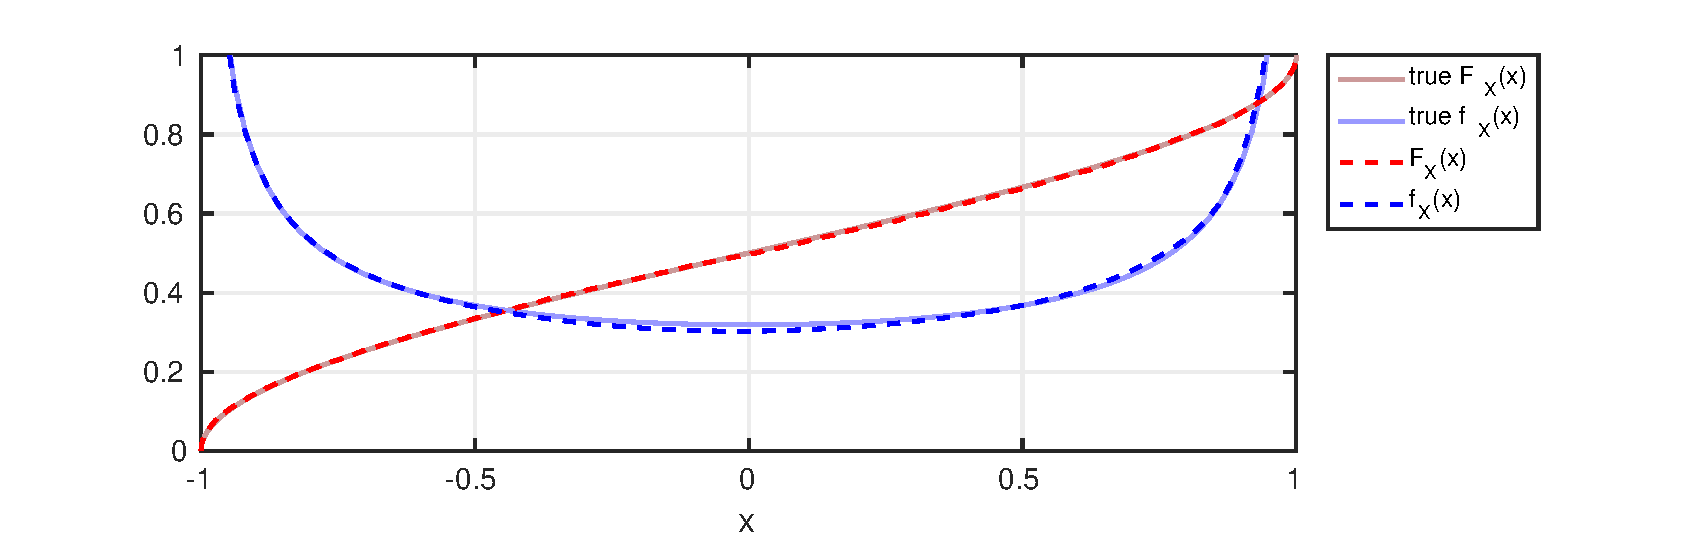
\includegraphics[width=\textwidth]{Prob1.eps}
\caption{Cumulative density function $F_X(x)$ and probability density function $f_X(x)$ based on analytical arguments and the inversion method using $N=10,\!000$ samples.}
\label{fig:prob1}
\end{figure}

%%%%%%%%%%%%%%%%%%%%%%%%%%%%%%%%%%%%%%%%%%%%%%%%%
%%%%%%%%%%%%%%%%%%%%%%%%%%%%%%%%%%%%%%%%%%%%%%%%%
\section*{Problem 2} %%%%%%%%%%%%%%%%%%%%%%%%%%%%
%%%%%%%%%%%%%%%%%%%%%%%%%%%%%%%%%%%%%%%%%%%%%%%%%
%%%%%%%%%%%%%%%%%%%%%%%%%%%%%%%%%%%%%%%%%%%%%%%%%

$G(x, \omega)$ is a Gaussian random process defined on $(0, 1)$. The mean and covariance functions of the Gaussian process $G(x, \omega)$ are
\begin{equation}
\xpect{G(x)} = 1.0, \qquad x \in (0,1),
\end{equation}
and
\begin{equation}
C_{GG}(x_1,x_2) = \sigma^2 \exp \left( \frac{- | x_1-x_2 | }{\ell} \right), \qquad (x1,x2) \in (0,1) \times (0,1),
\end{equation}
respectively. We would like to compute the eigen-pairs of $C_{GG}(x_1,x_2)$ using the Galerkin approach with linear finite elements (or the Nystr\"om approach) and compare them with the exact values provided in the notes.

For $(\sigma, \ell)$ of $(2,2)$ and $(2,0.2)$, we compute the number of terms required in the KL expansion of $G(x,\omega)$ such that the mean-square error of truncation is roughly 10\%. Then, we verify the increasing the finite element resolution reduces error of the Galerkin estimated eigenvalues. Finally, we draw 100,000 samples of the random process, plot seven of them, and compute the mean and variance of all samples, comparing them to the given values.

\subsection*{Methods}

Eigenvalues and eigenfunctions of the system are found by solving the generalized eigenproblem
\begin{equation}
\mathbf{C Z} = \mathbf{M Z \Lambda},
\end{equation}
where
\begin{equation}
\begin{aligned}
\mathbf{C}_{ij} &= \int_0^1 \int_0^1 C_{GG}(x_1,x_2) \; \psi_i(x_2) \; \psi_j(x_1) \; dx_1 dx_2 \\
\mathbf{M}_{ij} &= \int_0^1 \psi_i(x) \; \psi_j(x) dx \\
\mathbf{Z}_{ij} &= z_j^{(k)} \\
\mathbf{\Lambda}_{ij} &= \delta_{jk} \lambda_k
\end{aligned}
\vspace{1ex}
\end{equation}
are the matrices that result from the Galerkin formulation of the eigenvalue problem. In our case, we use piecewise linear basis functions $\psi_i(x)$, with $i = 1, 2, ..., N$. $\mathbf{M}_{ij}$ is computed analytically, and is proportional to the spacing between nodes in one-dimension, $\Delta x$. $\mathbf{G}_{ij}$ is computed on an element-wise basis in two-dimensions. The element-wise contributions to the integral are assembled in the standard manner.

These eigenvalues $\lambda_k$ and eigenfunctions $\phi_k(x)$ can be verified against the analytical solution presented in the course notes. With a sufficiently accurate eigenproblem solution, we can write the optimal orthogonal expansion of a random (not necessarily Gaussian) process as a Karhunen-Lo\`eve Expansion (KLE):
\begin{equation}
G_n(x,\omega) \equiv \sum_{i=1}^\infty \sqrt{\lambda_i} \phi_i(x) Y_i(\omega), \qquad
Y_i \widesim{iid} N(0,1).
\end{equation}

Since it is impractical to sum to $\infty$, only the first $d$ are used. One common way of determining a sufficient and practical cut-off $d$ is to reduce below some tolerance $\alpha$ the mean-square norm of the approximation:
\begin{equation}
d = \min_j \left\{ \frac{\sum_1^j \lambda_i}{\sum_1^\infty \lambda_i} \le \alpha \right\}
.
\label{eq:MSE_criterion}
\end{equation}

Finally, realizations of the random process are generated with
\begin{equation}
X(x) = \xpect{X(x)} + \sum_{i=1}^d \sqrt{\lambda_i} \phi_i(x) Y_i
.
\end{equation}

\subsection*{Discussion}

In \figref{fig:analytical_eigs}, we see that a longer correlation length $\ell$ is associated with a more rapid decay in eigenvalues. This is expected, since because more eigenfunctions are necessary to capture the higher-frequency dynamics of systems with small correlation length, their eigenvalues decay less rapidly.

In \figref{fig:error_reduction}, as expected, increasing the number of finite elements decreases the relative error of our approximated eigenvalues. The larger the magnitude of $\lambda_i$, the lower its relative error. Smaller correlation length $\ell$ corresponds to reduced eigenvalue accuracy for a given number of finite elements. Mathlab's `eigs` solver only solves for N-2 eigenpairs without producing warnings.

Finally, in \figref{fig:realizations}, we see the high-frequency behavior implied by smaller $\ell$ manifest in the seven individual realizations. For both $\ell=2$ and $\ell=0.2$, the sample mean matches the true mean very well; this is a direct consequence of reducing the mean square error to $<10\%$. The variance is less accurate, however. Larger $\ell$ results in a better approximation of variance, but this could be due to the mean-square error being reduced to 6.3\% for $\ell=2$, compared to 9.4\% for $\ell=0.2$. These are the highest values below 10\% for each case.

To investigate further, \figref{fig:realizations_moreterms} increases the KLE cutoff to include $b=17$ terms for the $\ell=0.2$ case, matching the $\ell=2$ case's MSE within 1\% using \eqref{eq:MSE_criterion}. Despite nearly identical MSE's, the $\ell=0.2$ variance is still $\sim2.5\%$ further away from the true value of $\sigma^2 = 4$ than the $\ell=2$ case's variance. I believe this results from variance being a higher-order statistic than the mean, which makes it inherently more difficult to capture with a small number of KLE terms. This effect is pronounced when the process has a shorter correlation length.

\begin{figure}[p]
\centering
\begin{subfigure}{0.49\textwidth}
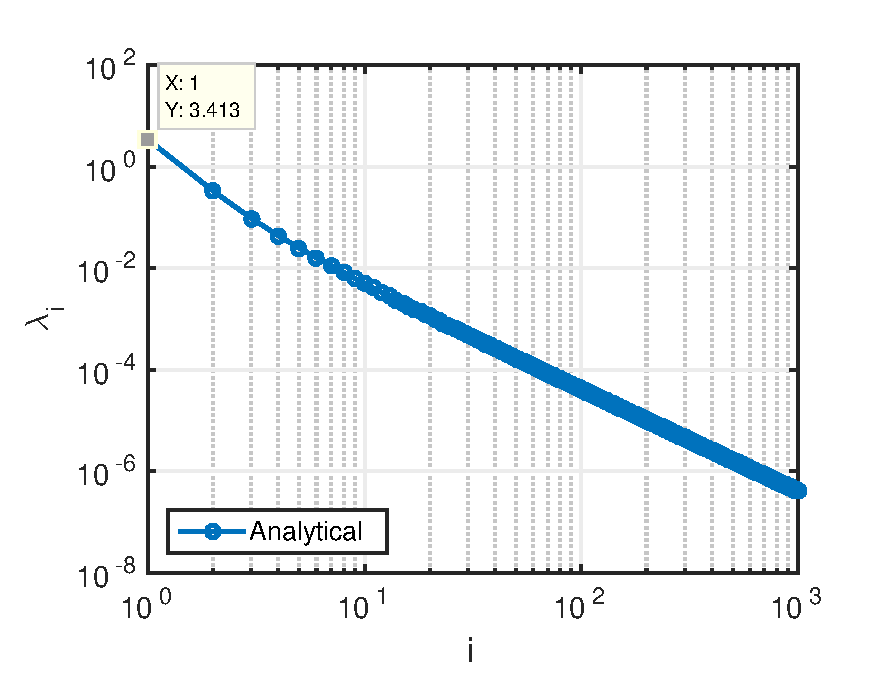
\includegraphics[width=\textwidth]{Prob2a1.eps}
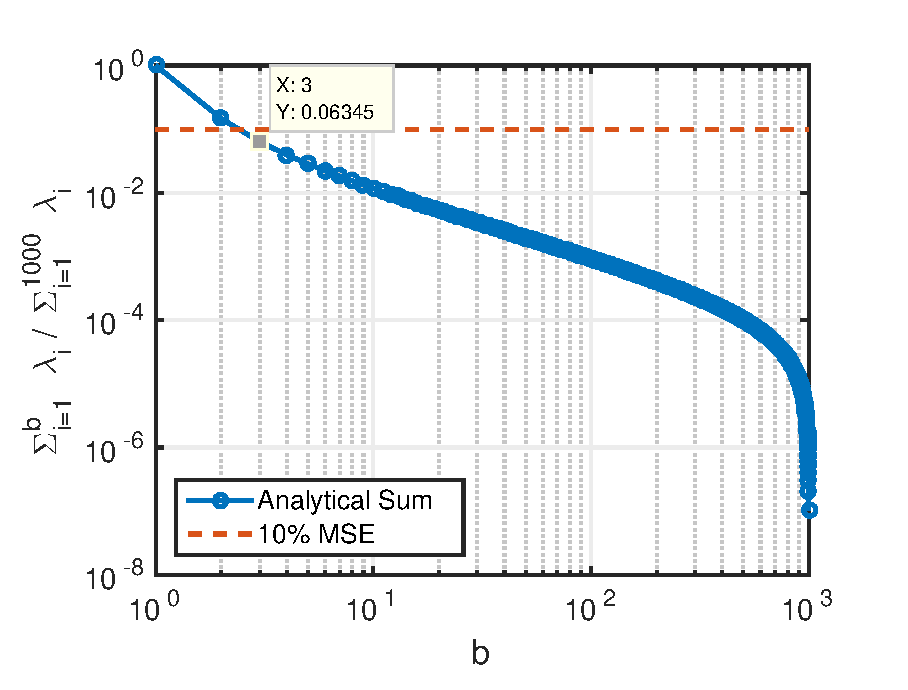
\includegraphics[width=\textwidth]{Prob2a2.eps}
\caption{$\ell=2$}
\end{subfigure}
\begin{subfigure}{0.49\textwidth}
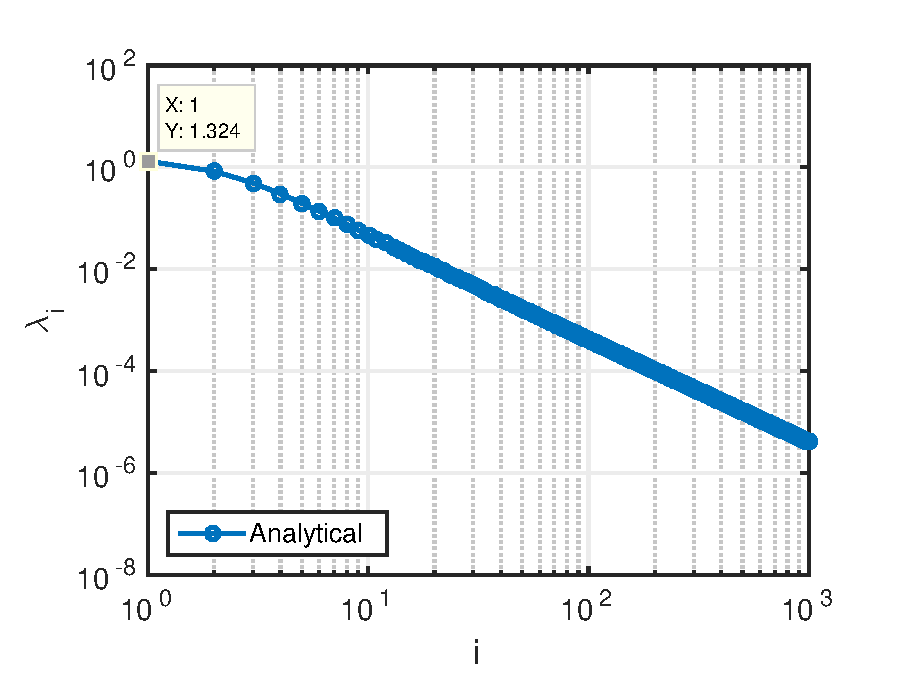
\includegraphics[width=\textwidth]{Prob3a1.eps}
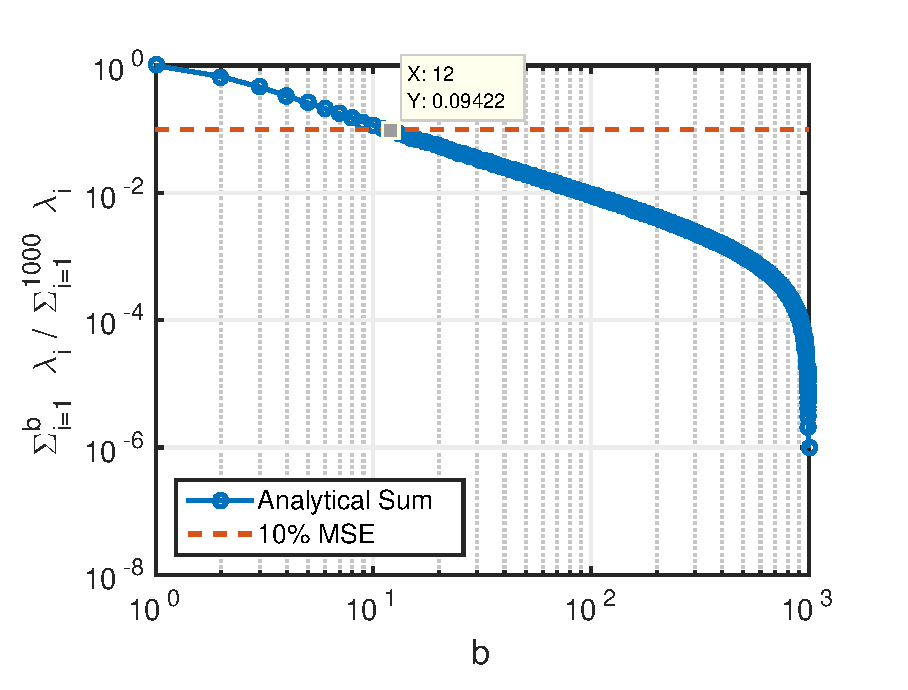
\includegraphics[width=\textwidth]{Prob3a2.eps}
\caption{$\ell=0.2$}
\end{subfigure}
\\[0.2cm]
\caption{1,000 analytical eigenvalues and normalized sum of the largest $b$ eigenvalues using $\sigma = 2$. Mean-square error of truncation $<10\%$ is first achieved with (a) $b=3$ and (b) $b=12$ terms in the KL expansion.}
\label{fig:analytical_eigs}
\end{figure}

\begin{figure}[p]
\centering
\begin{subfigure}{0.49\textwidth}
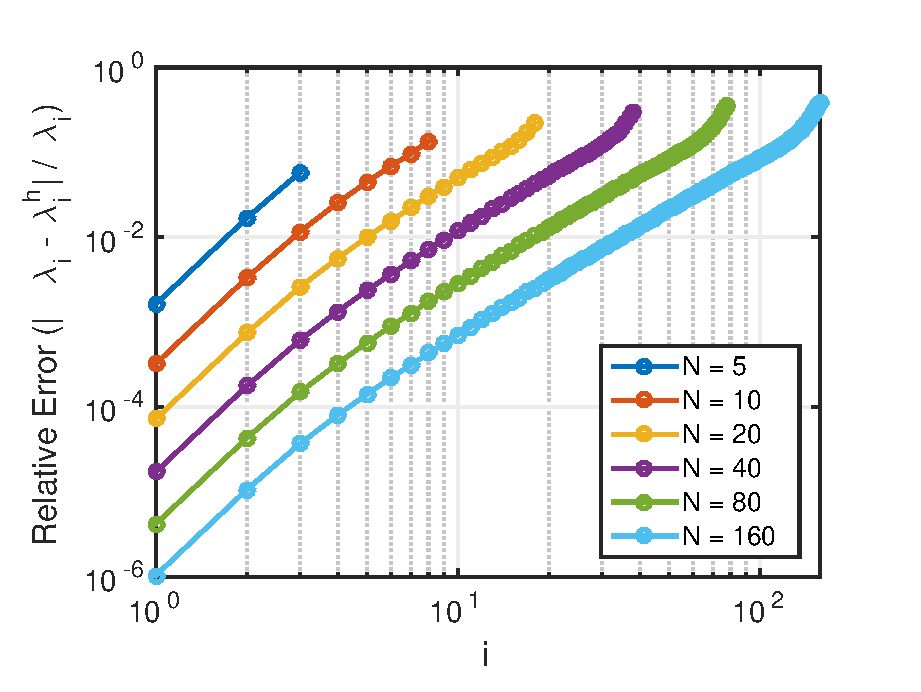
\includegraphics[width=\textwidth]{Prob2b.eps}
\caption{$\ell=2$}
\end{subfigure}
\begin{subfigure}{0.49\textwidth}
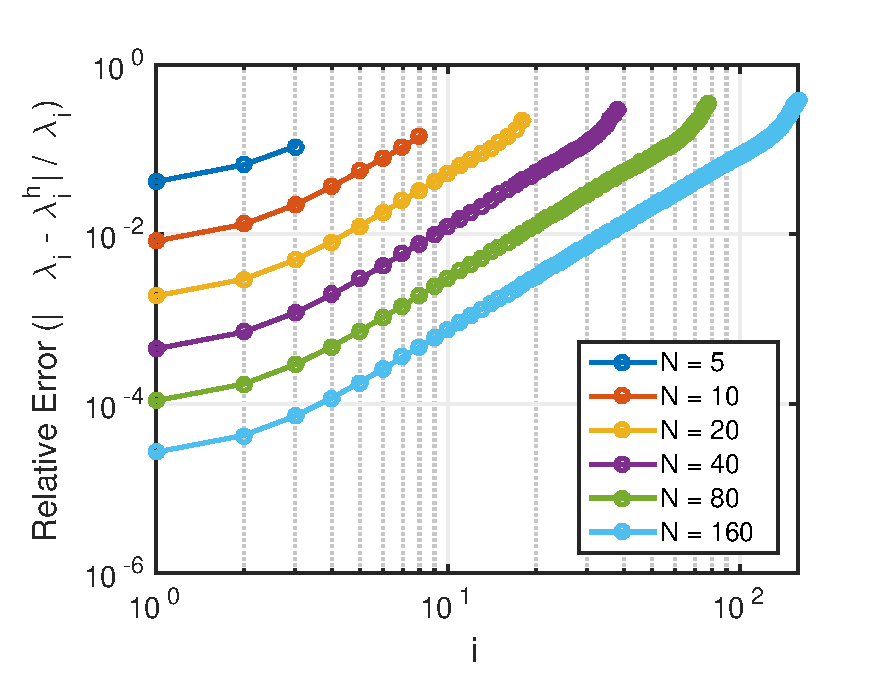
\includegraphics[width=\textwidth]{Prob3b.eps}
\caption{$\ell=0.2$}
\end{subfigure}
\\[0.2cm]
\caption{Increasing the number of finite elements ($N_\text{el}=[N-1]^2$) increases accuracy of eigenvalues. For both plots, $\sigma=2$.}
\label{fig:error_reduction}
\end{figure}

\begin{figure}[p]
\centering
\begin{subfigure}{0.49\textwidth}
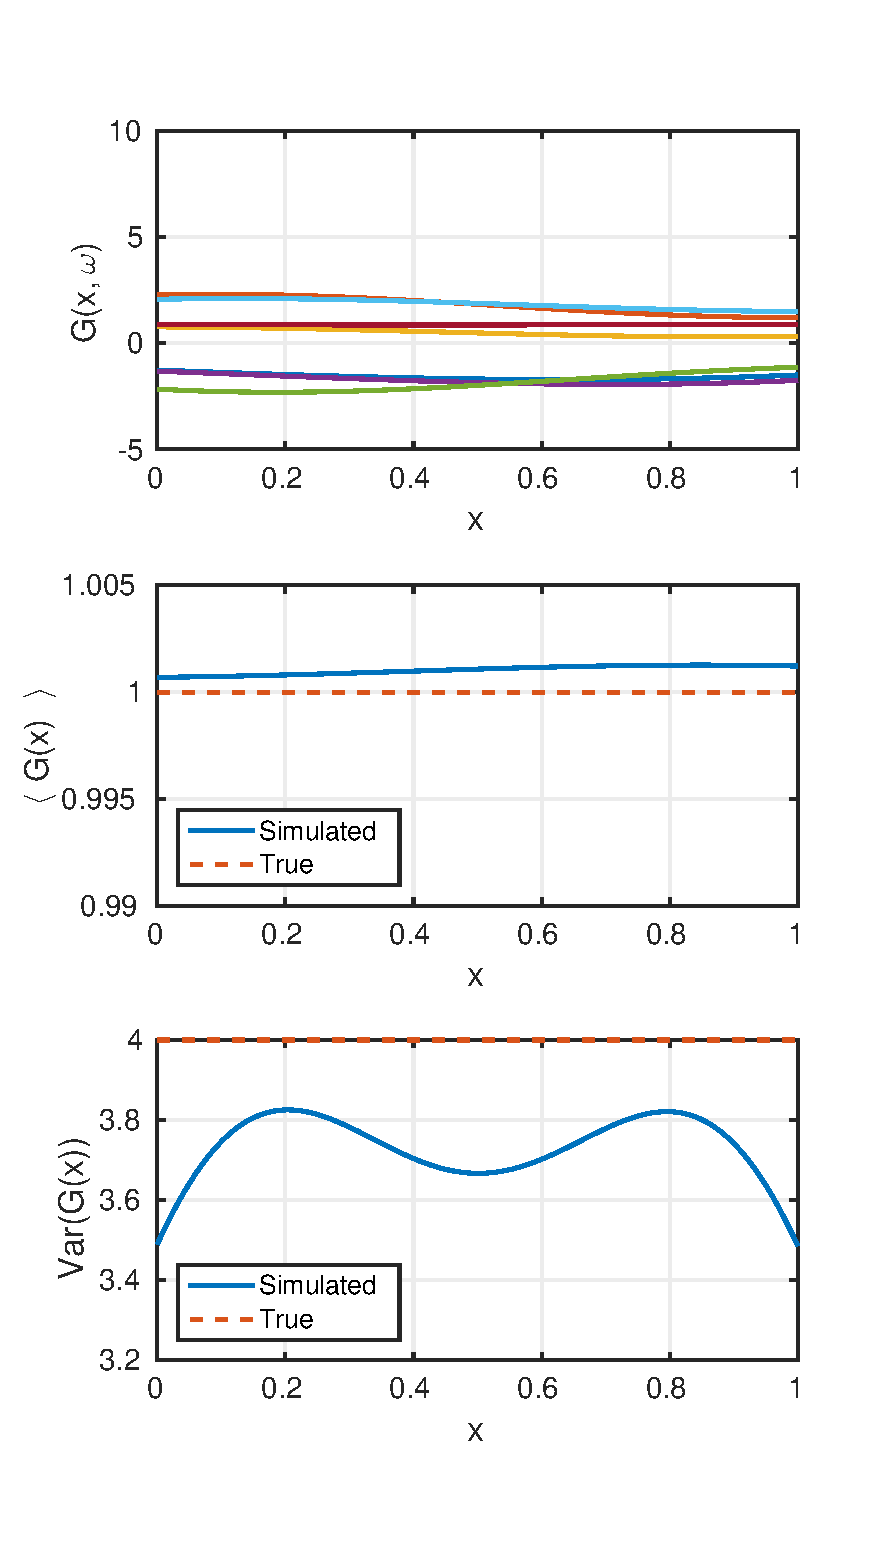
\includegraphics[width=\textwidth,trim={0 1cm 0 0}]{Prob2cd.eps}
\caption{$\ell=2$}
\end{subfigure}
\begin{subfigure}{0.49\textwidth}
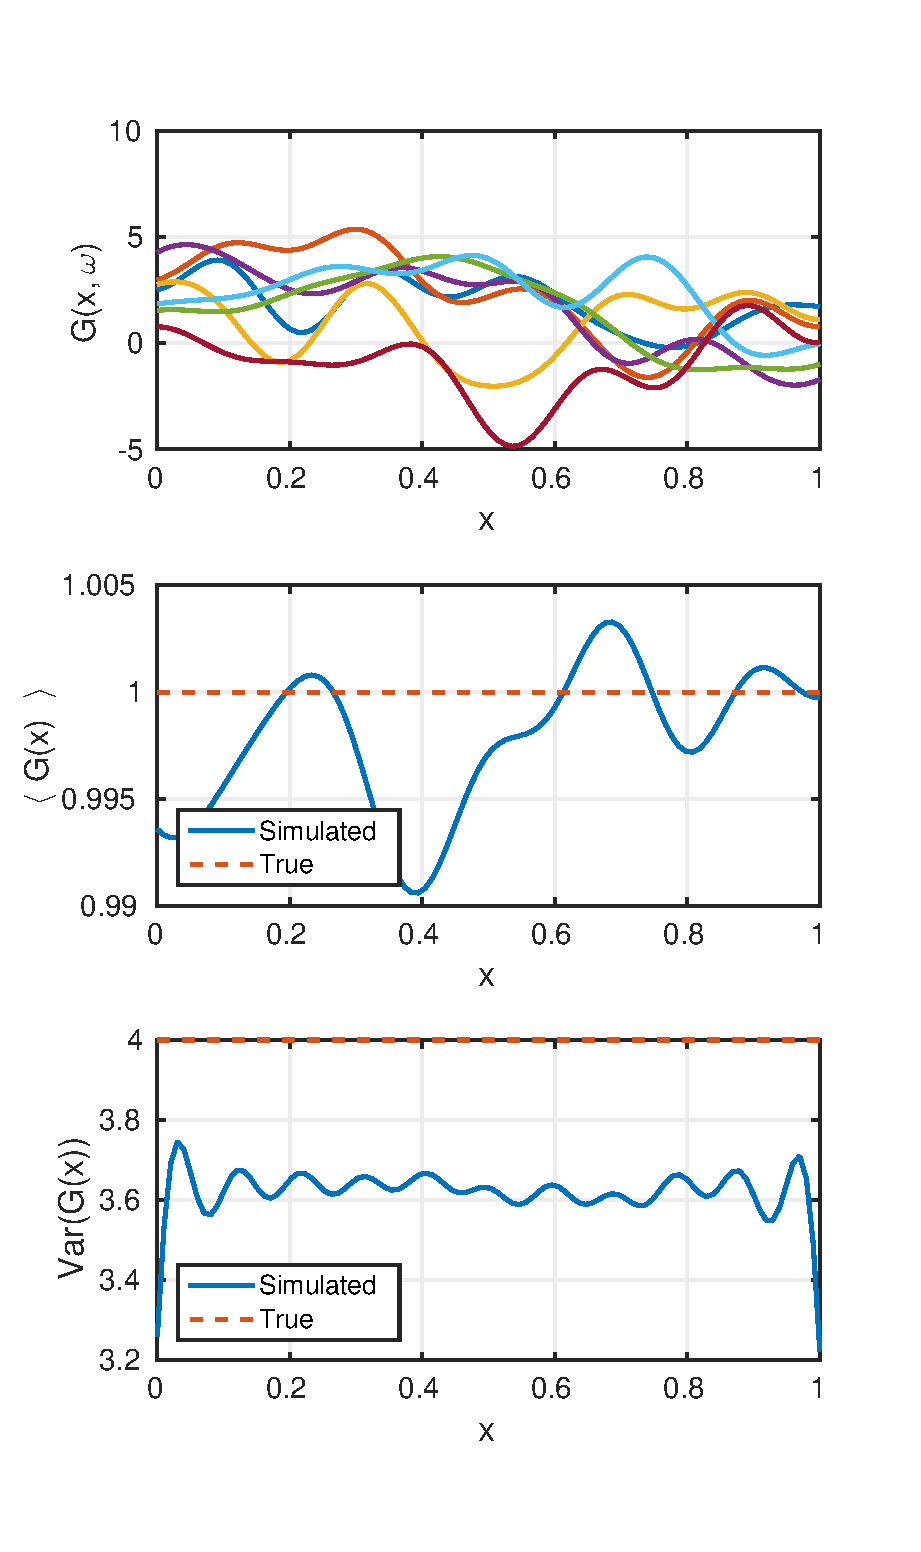
\includegraphics[width=\textwidth,trim={0 1cm 0 0}]{Prob3cd.eps}
\caption{$\ell=0.2$}
\end{subfigure}
\\[0.2cm]
\caption{From top to bottom: seven realizations of the random process $G(x,\omega)$, sample mean $\xpect{G(x)}$, and sample variance $\var(G(x))$, using 100,000 samples. For both plots, $\sigma=2$ and the KL expansion is used with $b(\ell)$ terms.}
\label{fig:realizations}
\end{figure}

\begin{figure}[p]
\centering
\begin{subfigure}{0.49\textwidth}
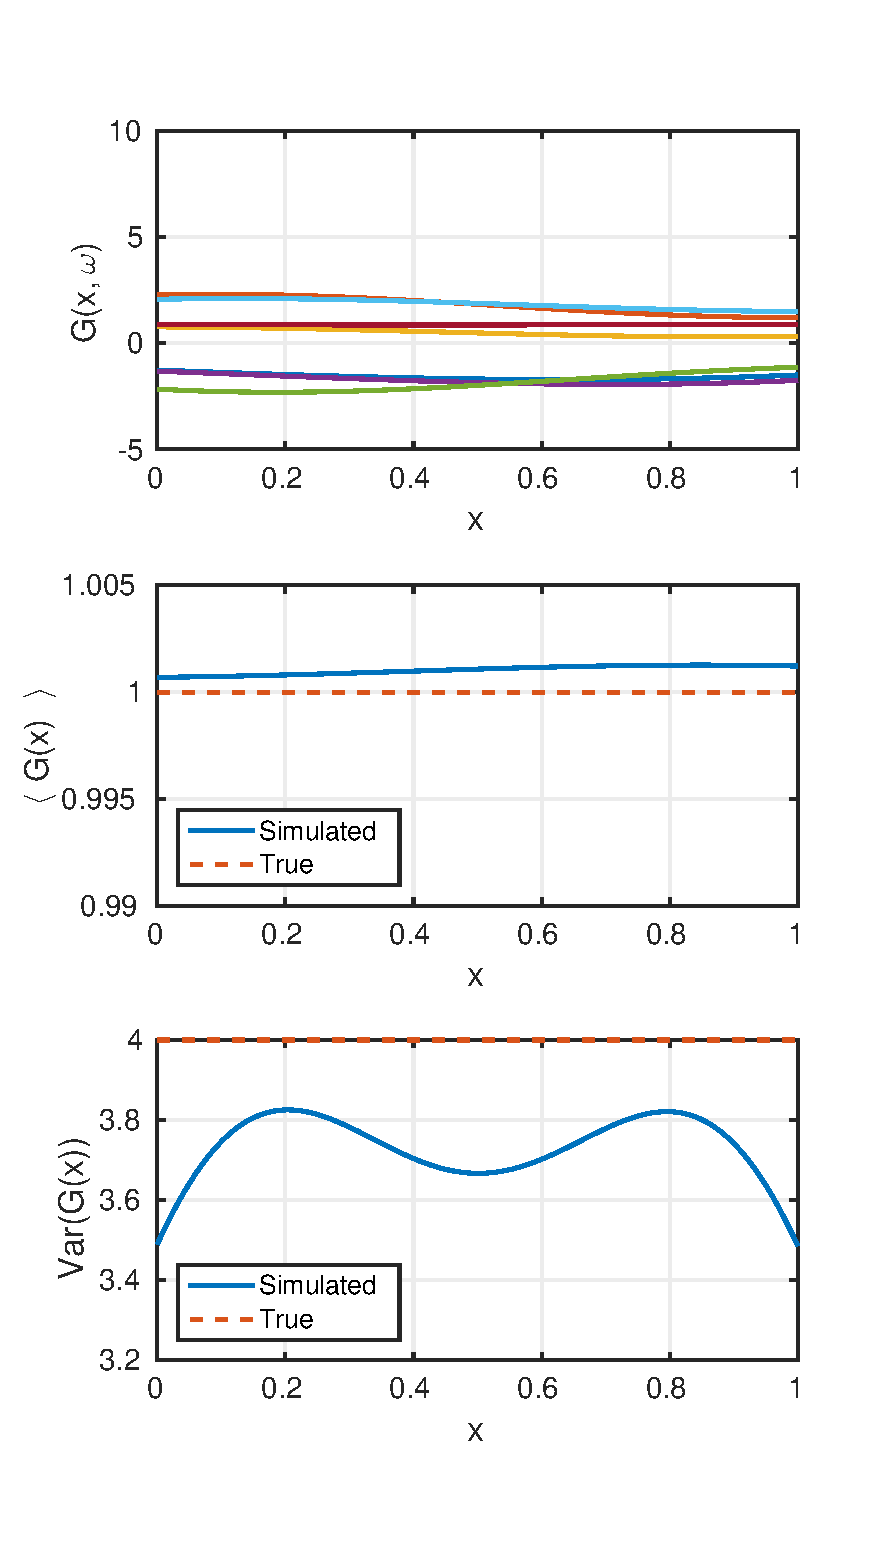
\includegraphics[width=\textwidth,trim={0 1cm 0 0}]{Prob2cd.eps}
\caption{$\ell=2$, MSE 6.34\%}
\end{subfigure}
\begin{subfigure}{0.49\textwidth}
\includegraphics[width=\textwidth,trim={0 1cm 0 0}]{Prob3cd_17terms.eps}
\caption{$\ell=0.2$, MSE 6.40\%}
\end{subfigure}
\\[0.2cm]
\caption{Same as \figref{fig:realizations}, but incorporating $b=17$ terms in the KL expansion of $\ell=0.2$ to match MSE with the $\ell=2$ case. For both plots, $\sigma=2$. Variance is still approximated better for case with longer correlation length.}
\label{fig:realizations_moreterms}
\end{figure}

%%
%% DOCUMENT END
%%
\end{document}
